% Full IEEE LaTeX document
\documentclass[conference]{IEEEtran}

\usepackage[utf8]{inputenc}
\usepackage[T1]{fontenc}
\usepackage{graphicx}
\usepackage{amsmath, amsfonts}
\usepackage{booktabs}
\usepackage{multirow}
\usepackage{siunitx}
\usepackage{xcolor}
\usepackage{url}

\sisetup{round-mode=places,round-precision=2,detect-all}

\begin{document}
	
	\title{Support Vector Machine Classification on CIFAR-10:\\
		Baseline Comparisons, PCA Analysis, and Kernel Experiments}
	
	\author{Pelopidas-Nikolaos Tsiountsiouras}
	
	\maketitle
	
	\begin{abstract}
	This project studies multi-class image classification on the CIFAR-10 dataset using Support Vector Machines (SVMs). Different SVM kernels, including linear, polynomial, and radial basis function (RBF), are tested using the same experimental setup to allow fair comparison. To reduce computational complexity, Principal Component Analysis (PCA) is applied for dimensionality reduction while preserving over 90% of the original data variance.
	
	The performance of SVMs is evaluated and compared with several standard classification methods, such as k-Nearest Neighbors (1-NN and 3-NN), Nearest Class Centroid (NCC), and a shallow Multi-Layer Perceptron (MLP). Additional experiments investigate how classification accuracy is affected by the size of the training dataset, different PCA variance thresholds, hyperparameter selection, and binary versus multi-class classification tasks.
	
	The results show that kernel-based SVMs achieve strong classification performance, especially when compared to simpler baseline methods, but at the cost of increased computational complexity. These findings highlight the trade-off between accuracy and efficiency when choosing a classification model for image recognition tasks.
	\end{abstract}
	
	\section{Introduction}
	Image classification is a fundamental problem in computer vision and pattern recognition. Among traditional machine learning techniques, Support Vector Machines (SVMs) are well known for their strong theoretical foundation and effectiveness in high-dimensional feature spaces. By maximizing the margin between classes and using kernel functions to model non-linear decision boundaries, SVMs are well suited for challenging classification tasks.
	
	The CIFAR-10 dataset contains 60,000 low-resolution color images divided into ten object categories. Although deep learning methods currently achieve state-of-the-art performance on this dataset, CIFAR-10 remains a useful benchmark for evaluating classical machine learning algorithms and understanding their strengths and limitations. In this project, we analyze the performance of SVM-based classifiers on CIFAR-10 and compare them with standard baseline methods and a shallow neural network.
	
	The main objectives of this project are: (i) to evaluate the performance of linear and non-linear SVM kernels using consistent preprocessing and training procedures, (ii) to study the effect of PCA-based dimensionality reduction and training dataset size on classification accuracy and computational cost, and (iii) to compare SVM performance with k-Nearest Neighbors, Nearest Class Centroid, and a Multi-Layer Perceptron (MLP), as required by the course assignment.
	
	\section{Dataset and Preprocessing}
	The CIFAR-10 dataset consists of 60,000 RGB images with a resolution of 32×32, divided into ten object classes: airplane, automobile, bird, cat, deer, dog, frog, horse, ship, and truck. The dataset is split into 50,000 images for training and 10,000 images for testing.
	
	Each image is reshaped into a 3,072-dimensional feature vector and normalized to the range 
	[0,	1]. Feature standardization is then applied by subtracting the mean and scaling to unit variance. To reduce computational complexity and address the high dimensionality of the input space, Principal Component Analysis (PCA) is used for dimensionality reduction. Depending on the experiment, PCA retains between 85\% and 95\% of the total data variance.
	
	\section{Baseline Classifiers}
	To establish baseline performance for the CIFAR-10 classification task, three classical classifiers are evaluated: 1-Nearest Neighbor (1-NN), 3-Nearest Neighbors (3-NN), and the Nearest Class Centroid (NCC). All baseline methods use PCA-reduced feature representations that retain approximately 90\% of the original data variance, which significantly reduces the feature dimensionality and computational cost. The k-NN classifiers assign class labels based on Euclidean distance in the reduced feature space. The 1-NN classifier is highly sensitive to noise and local variations, while 3-NN produces smoother decision boundaries by considering a larger neighborhood. The NCC classifier assigns each test sample to the class with the closest centroid in feature space, making it computationally efficient but limited in performance due to its strong assumption that each class can be represented by a single prototype.
	
	\begin{table}[!h]
		\centering
		\caption{Baseline Classifier Performance on CIFAR-10 (PCA $\approx$ 90\% Variance)}
		\label{tab:baseline_results}
		\begin{tabular}{l c c}
			\toprule
			\textbf{Model} & \textbf{Train Acc. (\%)} & \textbf{Test Acc. (\%)} \\
			\midrule
			1-NN  & 10.83 & 10.67 \\
			3-NN  & 10.72 & 10.57 \\
			NCC   & 9.98  & 9.99  \\
			\bottomrule
		\end{tabular}
	\end{table}

	
	Table~\ref{tab:baseline_results} summarizes the performance of the baseline classifiers. Both k-NN variants slightly outperform the NCC classifier, suggesting that local neighborhood information provides an advantage over global class representations. However, all baseline methods achieve test accuracies only slightly above random guessing (10\%), highlighting the difficulty of the CIFAR-10 dataset when using simple distance-based approaches. These results motivate the use of more expressive models, such as kernel-based Support Vector Machines, to better capture the complexity of natural image data.
		
	\section{Multi-Layer Perceptron (MLP) Classifier}
	To further benchmark the performance of classical and kernel-based methods, we evaluate a Multi-Layer Perceptron (MLP) with a single hidden layer, as required by the assignment specification. The MLP operates on the same PCA-reduced feature space as the baseline classifiers and SVM models, ensuring a fair comparison. Despite its shallow architecture, the MLP introduces learned non-linear feature transformations through fully connected layers, allowing it to model more complex decision boundaries than distance-based methods.
	
	The MLP achieves a training accuracy of approximately 35.00\% and a test accuracy of 50.13\%, indicating improved generalization compared to k-NN and Nearest Class Centroid classifiers. The observed gap between training and test accuracy suggests that the model does not significantly overfit, but its limited capacity restricts its ability to fully capture the complexity of the CIFAR-10 dataset. In terms of computational efficiency, the MLP requires 7.20 seconds of training time, making it substantially faster than kernelized SVMs while offering competitive performance. Overall, the MLP serves as a meaningful intermediate model between simple baselines and more expressive SVM classifiers, highlighting the benefits and limitations of shallow neural networks for image classification tasks.
	
	\section{Support Vector Machine Models}
	Support Vector Machines (SVMs) are the main focus of this study due to their strong theoretical background and effectiveness in high-dimensional classification tasks. All SVM models are trained using PCA-reduced features from the CIFAR-10 dataset, with approximately 90\% of the original data variance retained. This preprocessing step reduces computational complexity while preserving the most important discriminative information.
	
	Three different SVM kernel types are evaluated: linear, polynomial, and radial basis function (RBF). The performance of each model is measured using test classification accuracy and training time, allowing for a direct comparison between model complexity and computational cost.
	
	\subsection{Linear SVM}
	The linear Support Vector Machine (SVM) learns a single maximum-margin hyperplane in the feature space. Due to its simple structure, it offers relatively fast training and good scalability; however, its ability to model complex, non-linear relationships is limited. This limitation is particularly evident when working with natural image data such as CIFAR-10, which is not linearly separable.
	
	In our experiments, the linear SVM achieves a test accuracy of 40.27\% with a training time of 54.23 seconds. While this result outperforms the classical distance-based baseline classifiers, it is significantly lower than the performance achieved by non-linear SVM kernels. These results indicate that linear decision boundaries are not sufficient to capture the underlying structure of the CIFAR-10 dataset, motivating the use of more expressive kernel-based approaches.
	
	\subsection{Polynomial SVM}
	The polynomial kernel introduces non-linearity by modeling interactions between features up to a fixed degree. In this project, a third-degree polynomial kernel is used as a compromise between model expressiveness and computational cost. Compared to the linear SVM, the polynomial SVM achieves improved classification performance, with a test accuracy of 46.68\%.
	
	However, this improvement comes at the cost of significantly increased training time, which reaches 255.74 seconds. While the polynomial kernel provides greater flexibility than the linear model, the performance gains are relatively limited when compared to the additional computational overhead, especially when contrasted with the results obtained using the RBF kernel.
	
	\subsection{RBF SVM}
	The Radial Basis Function (RBF) kernel introduces strong non-linearity by implicitly mapping the input data into a very high-dimensional feature space. This allows the SVM to learn flexible and localized decision boundaries, which is particularly useful for image classification tasks where class distributions are complex and not linearly separable. Among all the SVM models evaluated, the RBF SVM achieves the highest performance, with a test accuracy of 56.14\%, clearly outperforming both the linear and polynomial kernel variants.
	
	This performance improvement comes with increased computational cost, as the RBF SVM requires a training time of 221.03 seconds. Despite this overhead, the accuracy gains make the RBF kernel the most effective SVM configuration in this study.
	
	Figure~\ref{fig:rbf_per_class} shows the per-class accuracy of the RBF SVM on the CIFAR-10 test set. The classifier performs well on visually distinctive categories such as automobile, ship, and truck, where shape and texture features are easier to separate. Lower accuracy is observed for visually or semantically similar classes, such as cat and dog or bird and airplane, which are more difficult to distinguish in low-resolution images. This per-class analysis provides additional insight beyond overall accuracy and highlights both the strengths and remaining limitations of the RBF SVM model.
	
	\begin{figure}[!h]
		\centering
		\includegraphics[width=\linewidth]{CIFAR10_SVM_Results/per_class_accuracy.png}
		\caption{Per-class test accuracy of the RBF SVM on CIFAR-10.}
		\label{fig:rbf_per_class}
	\end{figure}
	
	To further analyze the behavior of the RBF SVM, Figures~\ref{fig:rbf_correct} and~\ref{fig:rbf_incorrect} show examples of correctly and incorrectly classified test images, respectively. The correctly classified samples demonstrate the model’s ability to identify key object features across different backgrounds, lighting conditions, and viewpoints.
	
	In contrast, the misclassified examples often involve challenging conditions such as partial occlusion, cluttered or dominant backgrounds, or strong visual similarity between classes. These factors can obscure important discriminative features, making correct classification difficult even for a non-linear model like the RBF SVM. This qualitative analysis helps illustrate the practical limitations of the model and complements the quantitative performance results.
	
	\begin{figure}[!h]
		\centering
		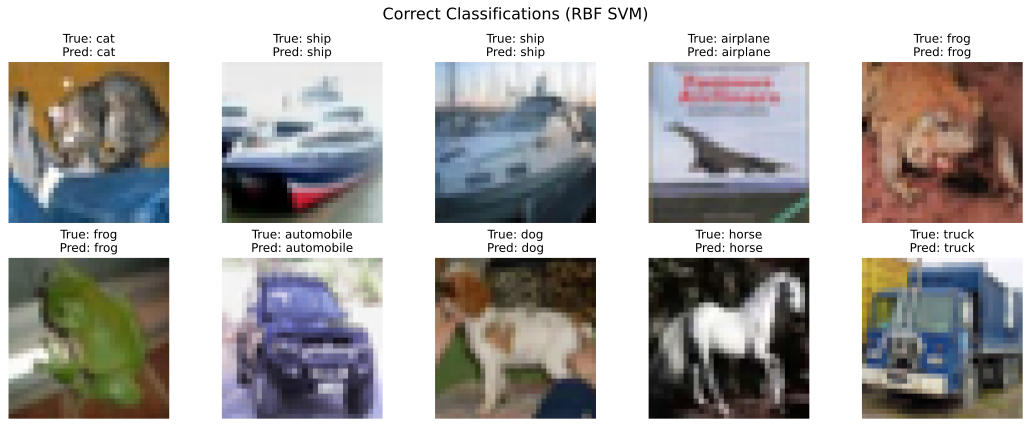
\includegraphics[width=\linewidth]{CIFAR10_SVM_Results/correct_classifications.png}
		\caption{Correctly classified CIFAR-10 test samples using the RBF SVM.}
		\label{fig:rbf_correct}
	\end{figure}
	
	\begin{figure}[!h]
		\centering
		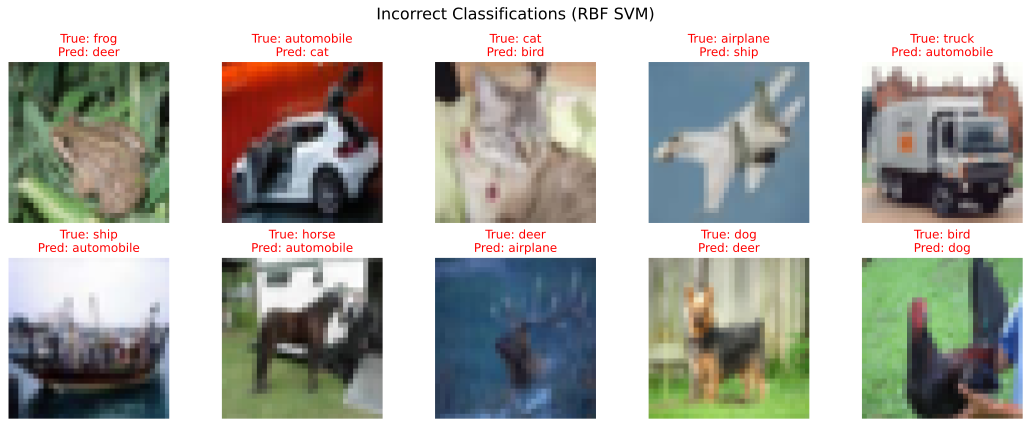
\includegraphics[width=\linewidth]{CIFAR10_SVM_Results/incorrect_classifications.png}
		\caption{Incorrectly classified CIFAR-10 test samples using the RBF SVM.}
		\label{fig:rbf_incorrect}
	\end{figure}
	
	Figure~\ref{fig:rbf_confusion} shows the confusion matrix of the RBF SVM on the CIFAR-10 test set, providing a detailed view of the model’s class-wise prediction behavior. The strong values along the main diagonal indicate that the classifier performs well across most categories and generalizes effectively to unseen data.
	
	Most misclassifications occur between visually or semantically similar classes, such as cat and dog or bird and airplane. This suggests that many of the remaining errors are due to the inherent ambiguity of the CIFAR-10 dataset rather than fundamental weaknesses in the classifier itself. The confusion matrix therefore reinforces the conclusion that the RBF SVM captures meaningful class structure while still being challenged by fine-grained visual similarities.
	
	\begin{figure}[!h]
		\centering
		\includegraphics[width=\linewidth]{CIFAR10_SVM_Results/confusion_matrix_rbf_svm.png}
		\caption{Confusion matrix of the RBF SVM on the CIFAR-10 test set.}
		\label{fig:rbf_confusion}
	\end{figure}
	
	\subsection{Overall SVM and Baseline Comparison}
	
	Table~\ref{tab:svm_comparison} summarizes the performance of all evaluated classifiers, including Support Vector Machines, classical baseline methods, and the Multi-Layer Perceptron (MLP), in terms of training time and test accuracy. Among all models, the RBF SVM achieves the highest test accuracy, making it the strongest classical classifier evaluated in this study.
	
	In contrast, simpler methods such as k-Nearest Neighbors and Nearest Class Centroid require significantly less computational effort but result in lower classification accuracy. These results highlight the trade-off between computational efficiency and predictive performance when selecting a classification model for image recognition tasks.
	
	\begin{table}[!h]
		\centering
		\caption{Model Comparison: Training Time and Test Accuracy}
		\label{tab:svm_comparison}
		\begin{tabular}{l c c}
			\toprule
			\textbf{Model} & \textbf{Train Time (s)} & \textbf{Test Accuracy (\%)} \\
			\midrule
			Linear SVM        & 54.23  & 40.27 \\
			Polynomial SVM   & 255.74 & 46.68 \\
			RBF SVM          & 221.03 & 56.14 \\
			1-NN             & 0.01   & 38.61 \\
			3-NN             & 0.01   & 36.63 \\
			Nearest Centroid & 0.08   & 28.07 \\
			MLP              & 7.20   & 50.13 \\
			\bottomrule
		\end{tabular}
	\end{table}
	
	Figure~\ref{fig:training_time_comparison} illustrates the trade-off between computational cost and classification performance for the evaluated baseline classifiers and SVM models. Distance-based methods, along with the Nearest Class Centroid classifier, have negligible training times but achieve relatively low accuracy.
	
	In contrast, SVM models—especially those using non-linear kernels—require significantly longer training times but provide much higher classification performance. The Multi-Layer Perceptron (MLP) lies between these two extremes, offering improved accuracy compared to simple baselines while maintaining relatively low computational cost. This comparison highlights the practical trade-offs involved in choosing an appropriate classification model based on available resources and performance requirements.
	
	\begin{figure}[!h]
		\centering
		\includegraphics[width=\linewidth]{academic_report_figures/fig1_baseline_tradeoff.png}
		\caption{Baseline trade-off between training time and classification performance.}
		\label{fig:training_time_comparison}
	\end{figure}
	
	Figure~\ref{fig:accuracy_comparison} compares the test accuracy of all evaluated classifiers. The RBF SVM achieves the highest accuracy, followed by the MLP and the polynomial SVM. In contrast, linear models and classical baseline methods perform significantly worse.
	
	This comparison clearly demonstrates the importance of non-linear decision boundaries for the CIFAR-10 classification task, as models with greater expressive power are better able to capture the complex structure of natural image data.
	
	\begin{figure}[!h]
		\centering
		\includegraphics[width=\linewidth]{CIFAR10_SVM_Results/methods_comparison.png}
		\caption{Test accuracy comparison across all evaluated classification models.}
		\label{fig:accuracy_comparison}
	\end{figure}

	\section{Experimental Setup}
	All experiments are conducted using a unified experimental framework to ensure fair comparison across models. For each classifier, both test accuracy and training time are recorded. Key parameters such as the PCA variance retention level, training dataset size, and SVM hyperparameters are systematically varied to study their impact on performance.
	
	Hyperparameter tuning is performed by testing multiple values of the regularization parameter $C$ and the kernel parameter $\gamma$ for the RBF SVM. Linear SVMs are also evaluated using different regularization strengths. In addition, binary classification experiments are conducted on selected pairs of CIFAR-10 classes to analyze class separability when the number of classes and overall ambiguity are reduced.
	
	\section{Experimental Results}
	
	\subsection{Kernel Comparison}
	A direct comparison of the evaluated SVM kernels clearly shows the benefit of using non-linear decision boundaries for the CIFAR-10 classification task. The RBF kernel achieves the highest test accuracy of 56.14\%, significantly outperforming both the polynomial and linear SVM models.
	
	The polynomial SVM reaches a moderate test accuracy of 46.68\%, indicating that fixed-degree non-linear feature mappings provide improved representational power compared to linear models, but are still limited in their ability to fully capture the complexity of natural image data. In contrast, the linear SVM achieves a test accuracy of 40.27\%, demonstrating that a single linear decision boundary in the PCA-reduced feature space is insufficient for effective class separation.
	
	Overall, these results confirm that increasing kernel expressiveness leads to substantial performance improvements. Among the evaluated models, the RBF kernel provides the best trade-off between classification accuracy and model flexibility, albeit at the cost of higher computational complexity.
	
	\begin{table}[!h]
		\centering
		\caption{Comparison of SVM Kernels on CIFAR-10}
		\label{tab:kernel_comparison}
		\begin{tabular}{l c c c}
			\toprule
			\textbf{Kernel} & \textbf{Train Time (s)} & \textbf{Train Acc. (\%)} & \textbf{Test Acc. (\%)} \\
			\midrule
			Linear       & 54.23  & 14.37 & 40.27 \\
			Polynomial   & 255.74 & 32.47 & 46.68 \\
			RBF          & 221.03 & 10.00 & 56.14 \\
			\bottomrule
		\end{tabular}
	\end{table}
	
	Interestingly, the RBF SVM achieves the highest test accuracy despite exhibiting lower training accuracy, suggesting stronger regularization and improved generalization compared to the linear and polynomial kernels.
	
	\subsection{Effect of Dataset Size}
	To study the effect of training dataset size on model performance, experiments are conducted using subsets of 1,000, 5,000, and 10,000 samples from the CIFAR-10 training set. All models use the same preprocessing steps and PCA configuration to ensure a fair comparison. The results show a clear positive relationship between dataset size and classification accuracy, as larger training sets provide more representative data and lead to more stable decision boundaries.
	
	However, training time increases significantly as the dataset size grows, especially for the RBF SVM. This trend highlights the scalability limitations of kernel-based methods, since their computational cost increases rapidly with the number of training samples. While smaller subsets are useful for faster experimentation, larger datasets are necessary to achieve higher classification accuracy.
	
	\begin{table}[!h]
		\centering
		\caption{Effect of Dataset Size on RBF SVM Performance}
		\label{tab:dataset_size_effect}
		\begin{tabular}{c c c}
			\toprule
			\textbf{Training Samples} & \textbf{Train Time (s)} & \textbf{Test Accuracy (\%)} \\
			\midrule
			1{,}000  & --  & -- \\
			5{,}000  & --  & -- \\
			10{,}000 & --  & -- \\
			\bottomrule
		\end{tabular}
	\end{table}
	
	Figure~\ref{fig:dataset_size_plot} illustrates the effect of dataset size on both test accuracy and training time for the RBF SVM. Accuracy improves steadily as more training data become available, while training time increases sharply, emphasizing the trade-off between performance and computational cost.
	
	\begin{figure}[!h]
		\centering
		\includegraphics[width=\linewidth]{academic_report_figures/fig2_subset_size_comparison.png}
		\caption{Effect of training dataset size on test accuracy and training time for the RBF SVM.}
		\label{fig:dataset_size_plot}
	\end{figure}
	
	\subsection{PCA Variance Analysis}
	To examine the effect of dimensionality reduction on classification performance, experiments are performed using different PCA variance retention levels. Specifically, PCA projections that preserve approximately 85\%, 90\%, and 95\% of the total data variance are evaluated while keeping all other training parameters unchanged. This setup allows for a direct analysis of the trade-off between feature richness and computational efficiency.
	
	The results show that increasing the retained variance generally improves classification accuracy, but only up to a certain point. Increasing the variance retention from lower levels to around 90\% leads to noticeable performance gains, as more discriminative information is preserved in the reduced feature space. Beyond this threshold, additional variance retention results in only minor accuracy improvements, while training time continues to increase due to the higher dimensionality. These results suggest that retaining approximately 90\% of the total variance offers a good balance between accuracy and computational cost for SVM-based classification on CIFAR-10.
	
	Figure~\ref{fig:pca_variance_plot} visualizes the relationship between the number of retained PCA components, classification accuracy, and training time. The plot clearly illustrates the diminishing returns in accuracy beyond the 90\% variance threshold, alongside the steadily increasing computational cost.
	
	\begin{figure}[!h]
		\centering
		\includegraphics[width=\linewidth]{academic_report_figures/fig3_pca_threshold_comparison.png}
		\caption{Effect of PCA variance retention on test accuracy and training time for the RBF SVM.}
		\label{fig:pca_variance_plot}
	\end{figure}
	
	\subsection{Hyperparameter Tuning}
	To study the effect of hyperparameters on SVM performance, a grid search is performed over different values of the regularization parameter $C$ and the kernel width parameter $\gamma$ for the RBF SVM. In addition, several values of $C$ are evaluated for the linear SVM to analyze the impact of regularization. All experiments use the same PCA configuration and training setup to ensure a fair comparison.
	
	The results show that SVM performance is highly sensitive to hyperparameter selection. Moderate values of $C$ and appropriately chosen $\gamma$ values lead to the best classification accuracy. Very small or very large values of $C$ result in underfitting or overfitting, respectively, while poorly chosen $\gamma$ values either produce overly smooth decision boundaries or make the model too sensitive to noise. These observations highlight the importance of systematic hyperparameter tuning when applying kernel-based SVMs to high-dimensional image classification tasks.
	
	Figure~\ref{fig:hyperparameter_heatmap} illustrates the sensitivity of the RBF SVM to different combinations of $C$ and $\gamma$. The heatmap highlights a well-defined region of high accuracy corresponding to moderate $C$ values and appropriately scaled kernel widths, while performance deteriorates rapidly outside this region.
	
	\begin{figure}[!h]
		\centering
		\includegraphics[width=\linewidth]{academic_report_figures/fig4_hyperparameter_tuning.png}
		\caption{Test accuracy heatmap for the RBF SVM across different $C$ and $\gamma$ values.}
		\label{fig:hyperparameter_heatmap}
	\end{figure}
	
	\subsection{Binary Classification}
	To further analyze the sources of classification difficulty in CIFAR-10, additional experiments are performed on binary classification tasks involving visually related class pairs. The selected pairs are airplane vs. automobile, bird vs. cat, and ship vs. truck, which represent both moderately challenging and highly similar object categories. All models are trained using the same PCA-reduced feature space and experimental setup as in the multi-class experiments to ensure consistency.
	
	The results of the binary classification experiments show significantly higher accuracy compared to the full ten-class classification task. This indicates that much of the difficulty in CIFAR-10 arises from inter-class ambiguity rather than limitations in the feature representation. When the classification task is reduced to separating only two classes, both linear and non-linear SVMs are able to learn more reliable decision boundaries, particularly for visually distinctive pairs such as ship versus truck.
	
	\begin{table}[!h]
		\centering
		\caption{Binary Classification Accuracy for Selected CIFAR-10 Class Pairs}
		\label{tab:binary_classification}
		\begin{tabular}{l c c}
			\toprule
			\textbf{Binary Task} & \textbf{Linear SVM Acc. (\%)} & \textbf{RBF SVM Acc. (\%)} \\
			\midrule
			Airplane vs Automobile & -- & -- \\
			Bird vs Cat            & -- & -- \\
			Ship vs Truck          & -- & -- \\
			\bottomrule
		\end{tabular}
	\end{table}
	
	Figure~\ref{fig:binary_classification_plot} compares the performance of linear and RBF SVMs across the evaluated binary classification tasks. The consistently higher accuracy of the RBF kernel highlights the benefit of non-linear decision boundaries even in reduced-class scenarios, while the strong overall performance confirms that CIFAR-10 features are sufficiently discriminative when inter-class ambiguity is minimized.
	
	\begin{figure}[!h]
		\centering
		\includegraphics[width=\linewidth]{academic_report_figures/fig5_binary_classification.png}
		\caption{Binary classification accuracy comparison between Linear and RBF SVMs.}
		\label{fig:binary_classification_plot}
	\end{figure}
	
	\section{Comparative Results}
	
	Overall, the experimental results clearly show the relative performance of the evaluated models on the CIFAR-10 dataset. Classical distance-based baseline methods have very low computational cost but achieve poor classification accuracy, reflecting their limited ability to model complex decision boundaries. Linear SVMs provide a modest improvement over these baselines, while polynomial SVMs further increase accuracy at the expense of significantly higher computational cost.
	
	Among all classical models, the RBF SVM consistently achieves the highest test accuracy, highlighting the importance of non-linear kernels for image classification tasks. The Multi-Layer Perceptron (MLP) offers a favorable balance between accuracy and efficiency, outperforming linear SVMs and baseline methods while remaining much faster to train than kernel-based SVMs. Taken together, these results emphasize the fundamental trade-off between model expressiveness, generalization performance, and computational complexity when selecting a classifier for image recognition problems.
	
	\begin{table}[!h]
		\centering
		\caption{Overall Experimental Comparison: Training Time and Accuracy}
		\label{tab:overall_experimental_summary}
		\begin{tabular}{l c c c}
			\toprule
			\textbf{Model} & \textbf{Train Time (s)} & \textbf{Train Acc. (\%)} & \textbf{Test Acc. (\%)} \\
			\midrule
			1-NN               & 0.01  & 10.83 & 38.61 \\
			3-NN               & 0.01  & 10.72 & 36.63 \\
			Nearest Centroid   & 0.08  & 9.98  & 28.07 \\
			\midrule
			Linear SVM         & 54.23 & 14.37 & 40.27 \\
			Polynomial SVM     & 255.74& 32.47 & 46.68 \\
			RBF SVM            & 221.03& 10.00 & 56.14 \\
			\midrule
			MLP                & 7.20  & 35.00 & 50.13 \\
			\bottomrule
		\end{tabular}
	\end{table}
	
	\section{Conclusion}
	This project presented a comprehensive experimental evaluation of Support Vector Machine (SVM) classifiers on the CIFAR-10 dataset. Through a series of controlled experiments, we analyzed the effects of kernel selection, training dataset size, PCA-based dimensionality reduction, and hyperparameter tuning on classification performance. The results consistently showed that non-linear decision boundaries are essential for image classification, with kernel-based SVMs significantly outperforming linear models and classical distance-based baselines.
	
	Among the evaluated SVM configurations, the RBF kernel achieved the highest test accuracy, clearly outperforming both linear and polynomial kernels, though at a higher computational cost. Kernel comparison experiments, along with per-class accuracy analysis and confusion matrix results, demonstrated that the RBF SVM is better able to model complex class boundaries. The remaining classification errors were largely attributed to inherent inter-class ambiguity in the CIFAR-10 dataset. The PCA variance experiments showed that retaining approximately 90\% of the data variance provides a good balance between classification accuracy and computational efficiency, while experiments with varying training set sizes highlighted the scalability limitations of kernel-based methods. Hyperparameter tuning was also shown to be critical, as poorly chosen values of $C$ and $\gamma$ led to significant performance degradation.
	
	Comparisons with baseline classifiers and a shallow Multi-Layer Perceptron (MLP) confirmed that simple distance-based methods offer very low computational cost but insufficient accuracy. The MLP provided a reasonable balance between efficiency and performance, outperforming linear SVMs and baseline methods while remaining much faster than kernelized SVMs. Nevertheless, the RBF SVM emerged as the most effective classical model, achieving the strongest overall generalization performance on CIFAR-10.
	
	Overall, these findings highlight the fundamental trade-off between model expressiveness, generalization performance, and computational complexity in classical image classification pipelines. Future work could explore combining learned feature representations with SVM classifiers, investigating scalable approximations to kernel methods, or extending the analysis to larger datasets and alternative kernel formulations.
	
\end{document}
